

\documentclass[main]{subfiles}

\begin{document}


\chapter{Methodology}

\section{Overview}

A panel of four local attribution methods were chosen for evaluation in this project, picked for representativeness of approach and their prominence in the literature. The panel was also a balanced selection from both `classes' of method approach: model-specific (Section \ref{sec:modelspec}) and model-agnostic (Section \ref{sec:modelag}):

\begin{enumerate}

\item \textbf{DeepLIFT:} Model-specific class, backpropagation-based approach (\ref{sec:backprop})
\item \textbf{GradCAM:} Model-specific class, gradient-based approach (\ref{sec:gradient})
\item \textbf{LIME:} Model-agnostic class, perturbation-based approach (\ref{sec:perturbag})
\item \textbf{SHAP:} Model-agnostic class\footnote{Due to its higher level formulation, SHAP has to be implemented for each model family. It's therefore better described as \textit{partially} model-agnostic.}, generic approach (\ref{sec:othermodelag})

\end{enumerate}

Other methods could have been included in this panel though as related work has shown in \ref{sec:existing_studies} (particularly by Ancona et al. (2017)), similarities in formulation should allow conclusions on one method to apply to close relatives. Project constraints also meant that a decision on the panel breadth had to be made according to at least some criteria, and representativeness helps for comparing approaches (the main project goal).

This chapter is presented in order of project milestones achieved, from initial data collection through to fine-tuning of the evaluation metrics designed. The evaluation methodology itself can be summarised in terms of the dataset used, `off the shelf' underlying models relied upon and the evaluation metric approach:
\newpage

\begin{enumerate}
\item \textbf{Dataset:} ImageNet validation set, with ground truth bounding box annotations usually used for object localisation training. 
\item \textbf{Models:} VGG16 as the primary model, InceptionV3 and ResNet50 for supportive analysis.
\item \textbf{Metrics:} Pixel-wise and mask-based WSOL, extending related work in Section \ref{sec:existing_criteria}.
\end{enumerate}

These are described in more detail in Sections \ref{sec:data}, \ref{sec:model} and \ref{sec:metric} below respectively. Finally, to support the metric analysis, qualitative analysis was also performed, though these results are left to the following chapter.


\section{Data Collection \& Annotation} \label{sec:data}

The ImageNet Large Scale Visual Recognition Challenge (ILSVRC) uses a subset of the well-known, hierarchically-labelled ImageNet database \cite{ilsvrc}. The competition's validation set consists of 50,000 images of 1000 categories, and includes annotations for ground truth class labels for image classification, and ground truth bounding boxes for object localisation.

This dataset was chosen because of the convenience of the bounding boxes for method evaluation, and the availability of models pre-trained on ImageNet. Images and bounding box XML files for all 50,000 instances in the 2012 validation set were acquired from an academically hosted torrent.

Each bounding box file contains one or several annotations (several if there are multiple instances of a single class, e.g. Figure \ref{dataimg}), and each annotation contains the ImageNet class ID and \{\textit{x-min, x-max, y-min, y-max}\} fields for the box\footnote{These ImageNet `synsnet' IDs were converted to human-readable class labels using a script that connects to a standalone map of IDs to labels.}.

A script to draw rectangular annotations on the images was created to sanity check the acquired data. Example outputs are shown in Figure \ref{dataimg}.

\begin{figure}[h]
\centering
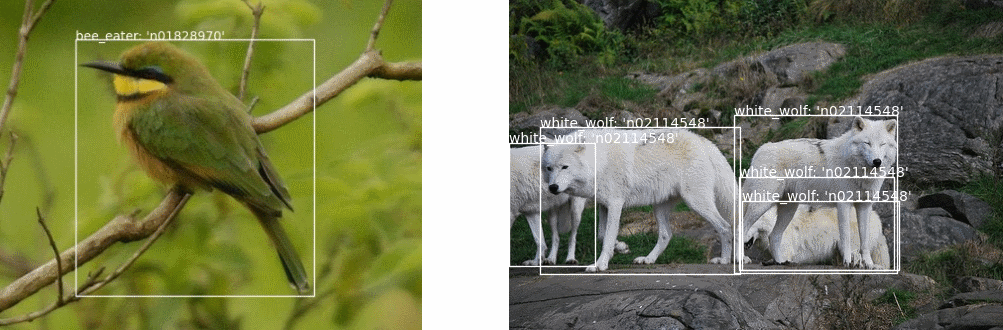
\includegraphics[scale=0.45]{annotation.png}
\caption{Collected ImageNet examples with annotations drawn.}
\label{dataimg}
\end{figure}

% caption PIL library was used

Much later into the project this script was upgraded to return the annotated image as a 2D array of 0's and 1's, with 1's inside the bounded regions to create a ground truth mask. The use of this mask for saliency calculation is described later (Section \ref{sec:metric}).

\section{Models \& Predictions} \label{sec:model}

Deep CNN models are expensive to train, so the high-level Keras library was used to import image classification models pre-trained on ImageNet \cite{keras}. Three models were chosen representative of common modern architectures (summarised in Table \ref{modeltable}). They acted as the underlying `black-box' models being explained.

\begin{table}[h]
\begin{tabular}{|l|l|l|l|}
\hline
\textbf{Model}       & \textbf{Structure}                                                                         & \multicolumn{1}{c|}{\textbf{Input Shape}} & \textbf{Project Role}  \\ \hline
\textbf{VGG16}       & \begin{tabular}[c]{@{}l@{}}16 stacked, 3x3 \\ convolutional layers\end{tabular}            & 224x224                                   & Most testing / results \\ \hline
\textbf{InceptionV3} & \begin{tabular}[c]{@{}l@{}}Stacked modules of \\ pooling + conv. layers\end{tabular}       & 299x299                                   & Supporting analysis    \\ \hline
\textbf{ResNet50}    & \begin{tabular}[c]{@{}l@{}}50-layer CNN with \\ `residual layer' connections.\end{tabular} & 224x224                                   & Supporting analysis    \\ \hline
\end{tabular}

\caption{Pre-trained image classifiers used in the project.}
\label{modeltable}
\end{table}

To check each model was working, a script was written to automate prediction collection and interact with preprocessed examples from the collected data. All software in the project was developed to be agnostic about the underlying model, though some methods required specific hyperparameters like a layer target. These targets were set up in a high level struct-type object in a constants file.

\section{Software Abstraction I}  \label{sec:sw1}

Each model requires input resizing and preprocessing in some form. An \textit{ImageHandler} class was therefore designed to abstract from complexity related to different representations of a single image instance. All input/output file methods and getter methods for raw, expanded and preprocessed representations were stored in this class, which made enforcing model agnosticity and adapting methods (Section \ref{sec:adaption}) much easier.


\newpage
\section{Initial Method Investigation}  \label{sec:initial}

Public GitHub implementations for each of the four methods were sourced: GradCAM \cite{gradcamrepo}, DeepLIFT \cite{deepliftwrapperrepo}, SHAP \cite{shaprepo} and LIME \cite{limerepo}.

They were then run on some high-confidence instances fed into the VGG16 model (correct predictions with p $>$ 0.75) and their `out of the box' saliency maps were then visually inspected. Examples are shown in Figure \ref{panelimg} over the page. Note  different method formulations result in different explanatory features being highlighted, even for the same example and model prediction. Some other initial observations on each method were made:

\begin{itemize}
\item \textbf{GradCAM:} The heatmap represents the localisation characterised in the target layer (final convolutional layer). The Guided GradCAM variant (Section \ref{sec:gradient}) was later used instead for a more discriminative version of the same saliency map.
\item \textbf{DeepLIFT:} Attributions are relatively `noisy', emphasise edges, and are higher resolution due to being being captured in the original input shape.
\item \textbf{SHAP:} Attributions are in the shape of the input to a target hidden layer, which accounts for its lower resolution. 
\item \textbf{LIME:} The method represents connected component `super pixels' as the explanatory features, though in Figure \ref{panelimg} these appear patchy on the maze-like patterns on the coral, the texture of the hair on the monkey's face, and the wheat in the field.
\end{itemize}


\begin{figure}[htbp]
\centering
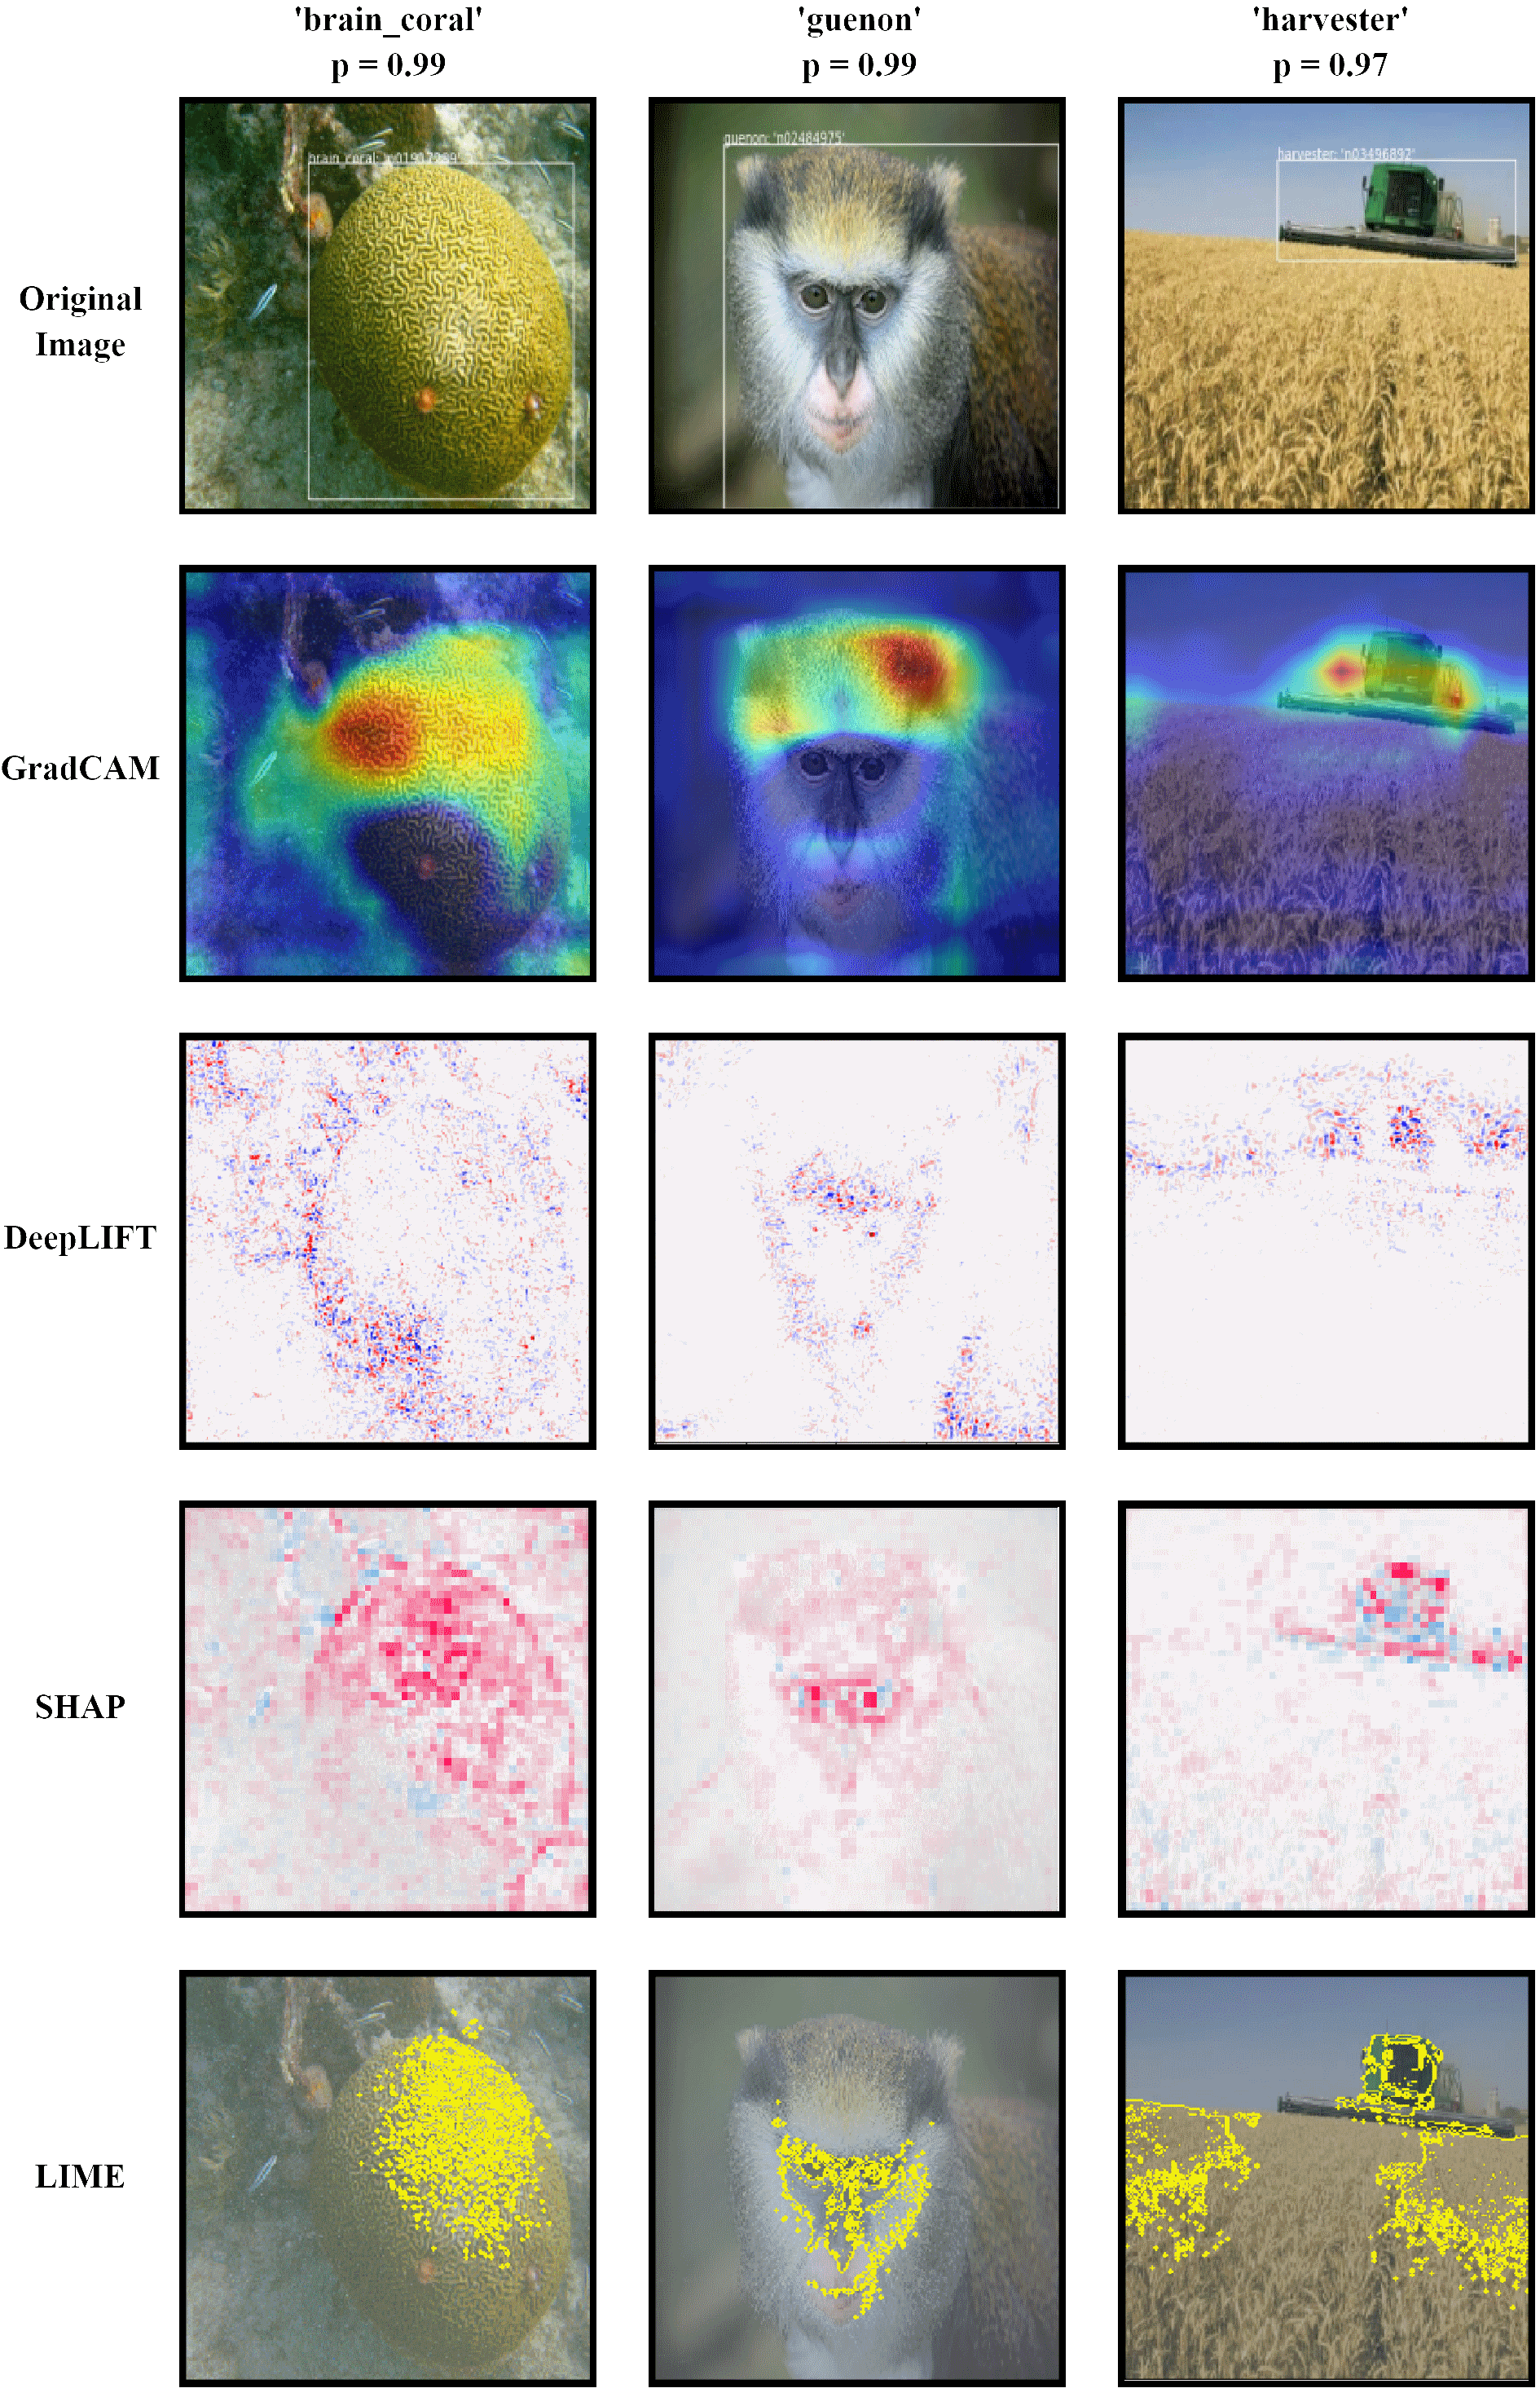
\includegraphics[scale=0.28]{method_box.png}
\caption{Default attributions for methods applied to high-confidence VGG16 predictions (class label and softmax output at top). Original image is resized with annotation drawn for reference. }
\label{panelimg}
\end{figure}

\section{Software Abstraction II}  \label{sec:sw2}

Each method was wrapped in its own class with an \textit{attribute()} function to return the array that represented its explanation output. Repeated logic in each method's implementation was also extracted into an \textit{Attributer} class fitted over these methods. This was a helpful prerequisite to adapting the methods for comparison. The functions in this class visualise figures, save returned NumPy arrays to results files, apply a colour map to highlight positive / negative attribution weights and the intensity of those weights, and normalise attributions between -1 and 1. This class is included in Appendix A and referred to in the class diagram in Figure \ref{sec:sw2}.

\newpage
\section{Adapting Methods for Compatibility}  \label{sec:adaption}

Some methods had higher level implementations than others (SHAP and DeepLIFT) in the code. For example, the output representation of SHAP was generated in internal methods that made it necessary to implement modified functions that overrode method internals. Others did not hide internal logic and were easier to adapt.

Visual examples of the methods made compatible for evaluation are shown in Figures \ref{panel2img} and \ref{panel3img}. Some brief comments  about work necessary for each method and the insights gained:

\begin{itemize}
\item \textbf{GradCAM:} Guided GradCAM required very little adaption, since the attributions were already in the shape of the input feature space. Support for specifying the final conv. layer (target for each model architecture) was added.
\item \textbf{DeepLIFT:} Similar to GradCAM, the only changes made for DeepLIFT were to change the colour map function and extract logic into the \textit{Attributer} class.
\item \textbf{SHAP:} These attributions had to be resized into the shape of the input feature space. Initially the smaller dimensions were dealt with by scaling them up and using an interpolation method from the OpenCV library. However, this led to biased results from the `blur' effect of the interpolation. To replace that workaround, the attribution was multiplied with a Guided Backpropagation output following the Guided GradCAM approach.
\begin{figure}[htbp]
\centering
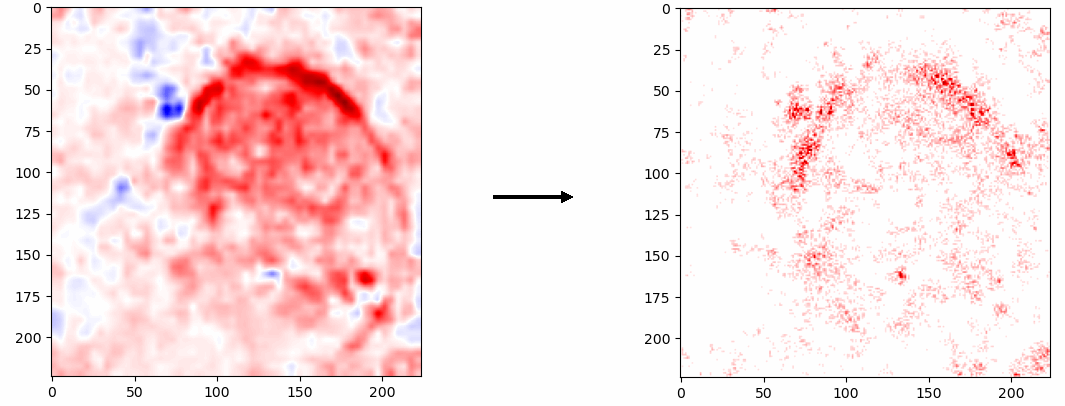
\includegraphics[scale=0.3]{shap_change.png}
\caption{Blurred workaround for SHAP versus the improved approach.}
\label{panelimg}
\end{figure}


\item \textbf{LIME:} To obtain per-pixel attributions from the super pixel regions, the linear model weights on each super pixel (output by an internal LIME method) were applied to a mask over the region bounded by each super pixel. This is a change in the interpretation of the authors' method, though it was necessary to obtain attribution weights.
\end{itemize}

Importantly, support for thresholding the attributions in terms of standard deviations was added at this point. An optional parameter was also implemented to have attributions returned with the absolute value taken, to take positive and negative evidence together as simply evidence.

\begin{figure}[htbp]
\centering
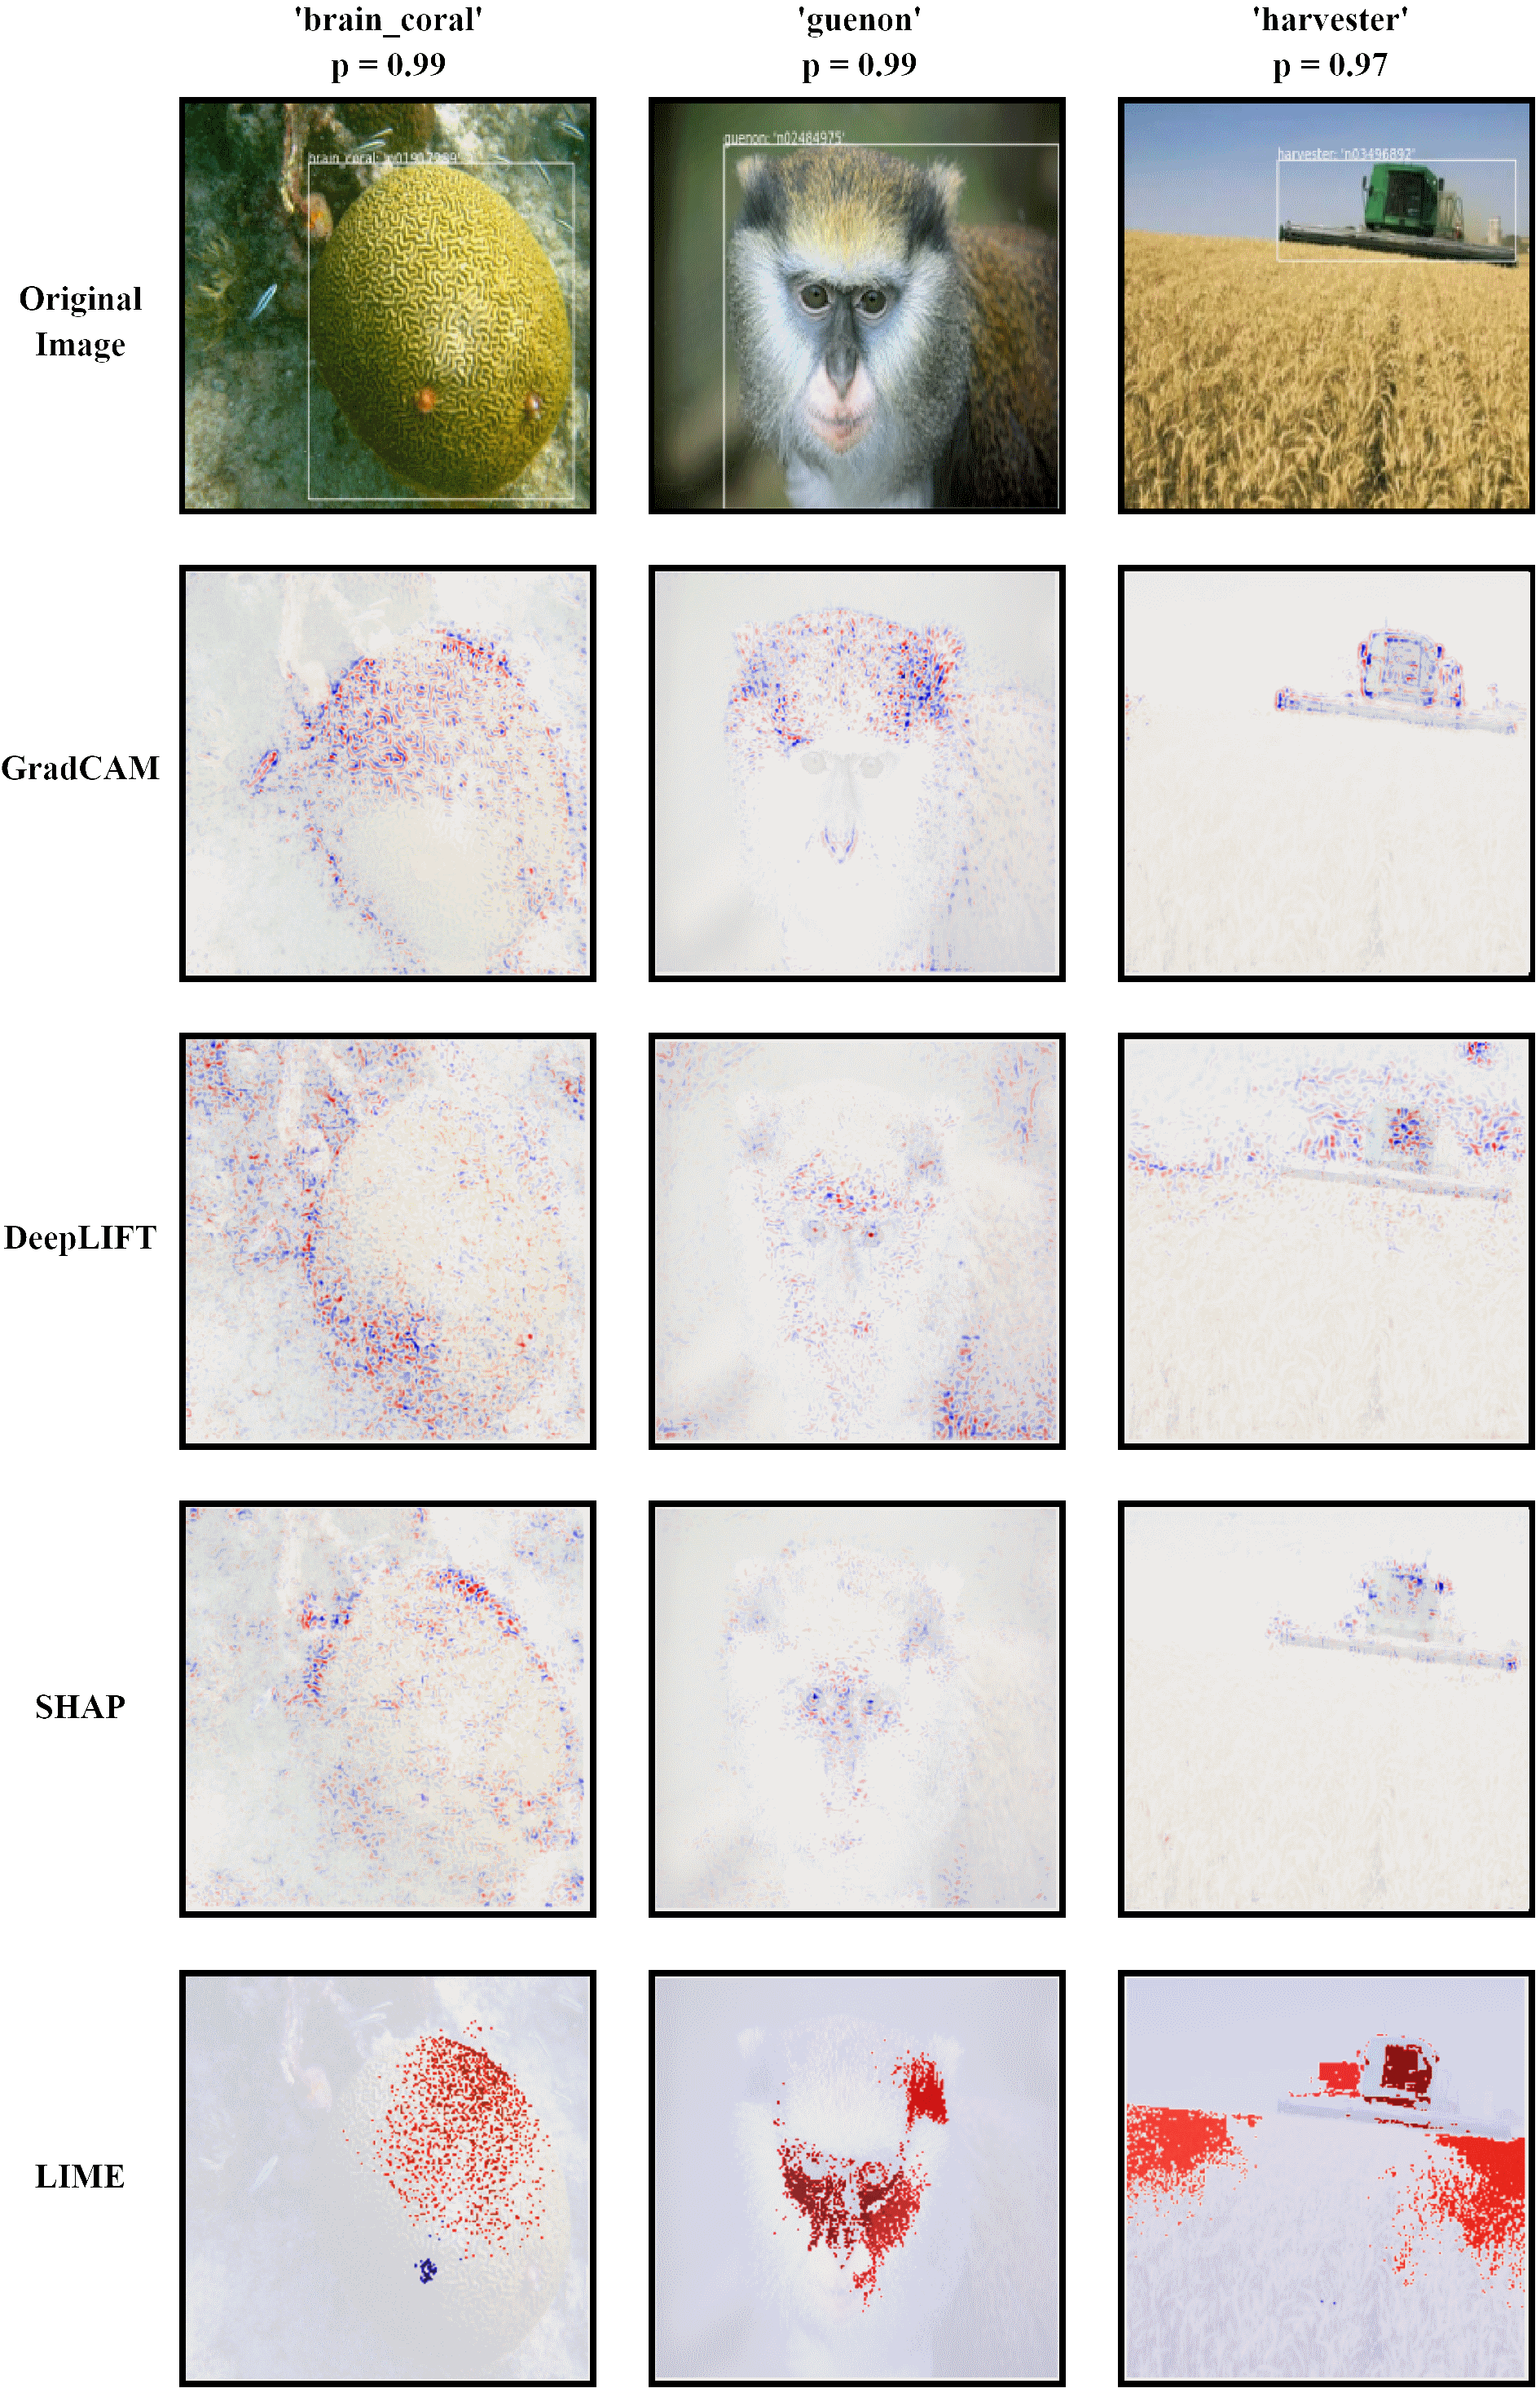
\includegraphics[scale=0.28]{method_box_adapted_1.png}
\caption{Adapted attributions for methods applied to high-confidence VGG16 predictions (original image faintly imposed). Each is a 2D, input-space-sized Numpy array that is normalised between -1 and 1 for the pixel attribution weights / entries in the array. Positive evidence/weights are in red and negative evidence is in blue, and darker colours indicate larger weights / `stronger' evidence.}
\label{panel2img}
\end{figure}



\begin{figure}[htbp]
\centering
\includegraphics[scale=0.2]{method_box_adapted_2.png}
\caption{Adapted attributions with absolute value taken and a threshold of one standard deviation applied.}
\label{panel3img}
\end{figure}


\newpage


\section{Evaluation Metric Design} \label{sec:metric}

In Section \ref{sec:existing_criteria} it was argued that existing saliency metrics in the literature do not account for pixel-level saliency via feature weights, and the approach to generate bounding boxes via single-component segmentation can unfairly punish perforated-looking saliency maps. Figures \ref{panel2img} and \ref{panel3img} also show that the adapted method outputs are discriminatory and fine-grained, rather than localising and coarse-grained, which adds a further motivation for a more suitable metric than the connected-component approach for WSOL. The two metrics designed were both based on intersection-over-union though calculated over individual pixels rather than boxes:

\begin{enumerate}
\item \textbf{Pixel-wise IOU:} A mask of the instance's ground truth bounding box is compared with the 2D array of each method's saliency map (example in Figure \ref{iou_example_img}). Weights are ignored and pixels are counted as intersecting if they have a value in both arrays. The intersection array's area is divided by the union array's area to generate the result.
%$\frac{Saliency Map \cap Annotation Mask}{Saliency Map\cup Annotation Mask}$

\item \textbf{Pixel-wise IOU*:} A variant to account for intensity of attribution / weights on each pixel. Instead of 1s in the intersection array the attribution weight is directly stored (with absolute value taken). The union array (denominator) is unchanged. This was a purely intuitive measure to crudely reward intensity of attribution and punish methods that provide uncertain or `non-commital' explanations with low attribution weights.

\end{enumerate}

This approach to explanation quality is different from the localisation performance approach of others and results in much lower IOU (though this is not as concerning since there is consistency across the panel). Related work introducing \textit{individual} methods did care about IOU magnitude to be able to use ILSVRC object localisation competitors as benchmarks for evaluating their own method.

\begin{figure}[htbp]
\centering
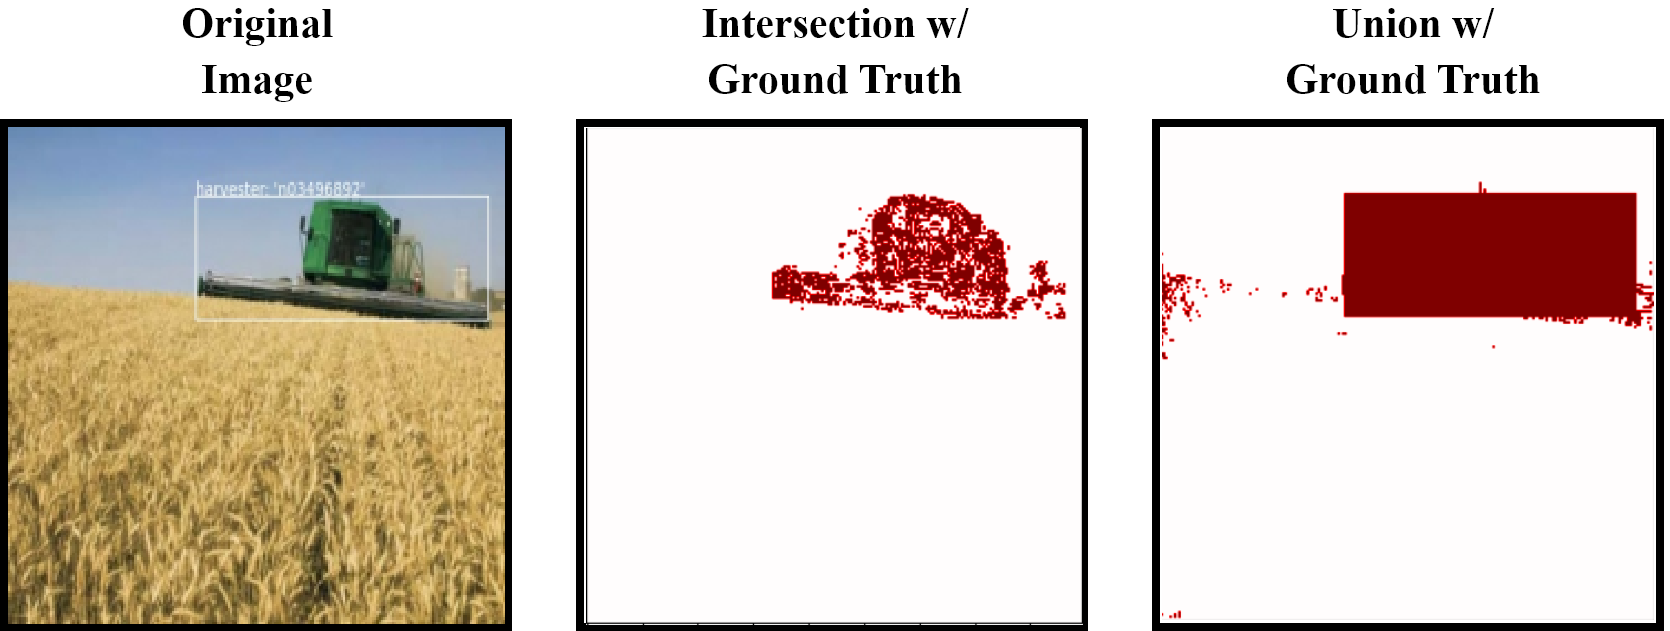
\includegraphics[scale=0.22]{iou_example.png}
\caption{Example IOU calculation for a GradCAM attribution  (=0.33). Threshold of one standard deviation is applied to the attribution before calculation.}
\label{iou_example_img}
\end{figure}

\newpage

The design of a proxy metric was meant to provide only some objective basis for evaluating methods in the image classification context. Other analysis was also performed for testing methods on higher level criteria than only IOU saliency (Results chapter).

%Performance wise, it is more taxing to account for pixel-wise attribution

\section{Software Abstraction III}  \label{sec:sw3}

To collect IOU and IOU* evaluations over many instances an \textit{Evaluator} class was developed that implements the following functions:
\begin{enumerate}
\item Collect annotation mask for an instance, and a method's output attribution
\item Calculate IOU and IOU* for a given annotation mask and attribution
\item Append results to a dataframe and periodically write to a CSV file
\item Perform the above for batches of instances and for the full method panel
\end{enumerate}

The class can potentially implement other saliency metrics, as IOU and IOU* are modularised functions.

\begin{figure}[htbp]
\centering
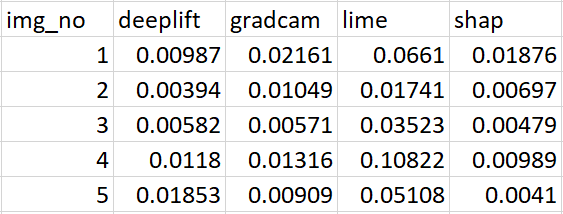
\includegraphics[scale=0.4]{csv_output.png}
\caption{CSV excerpt of a results batch file for IOU metric data.}
\label{csv_image}
\end{figure}

Finally an \textit{Analyser} class was created to read the collected CSV data, calculate statistics (means and standard deviations), and generate graphs for any subset of methods or metrics. Example graphs are shown in the Results chapter.

The descriptions in Sections \ref{sec:sw1}, \ref{sec:sw2} and this section of the developed testing framework are summarised in Figure \ref{flow_image}. The \textit{Attributer} and \textit{Evaluator} classes are included in \textbf{Appendices A and B} respectively.


\begin{figure}[htbp]
\centering
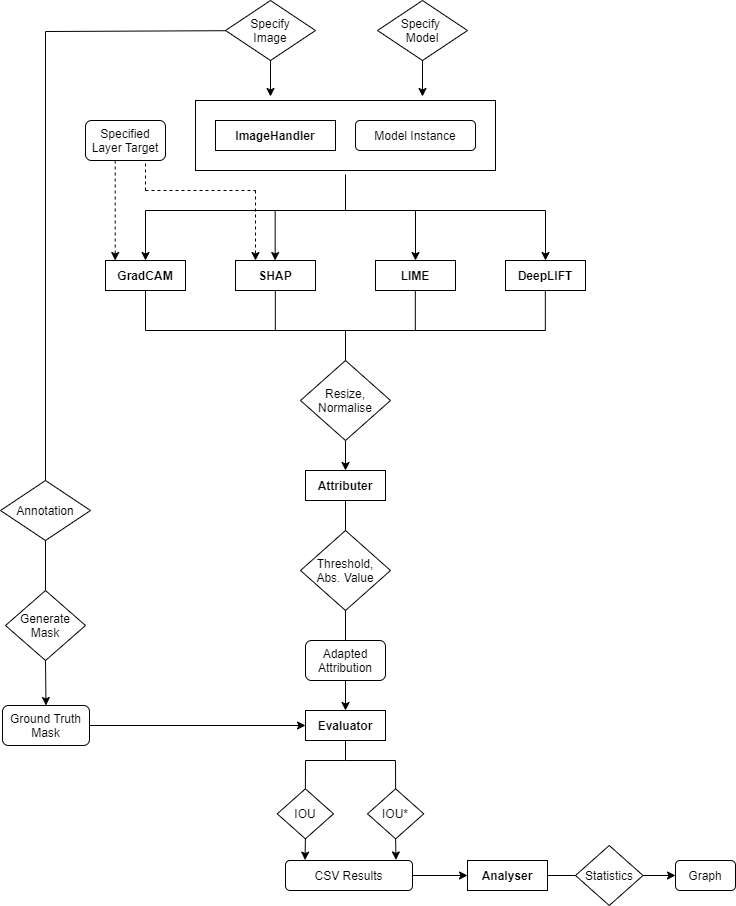
\includegraphics[scale=0.6]{program_flow.png}
\caption{High-level flow diagram of testing framework.}
\label{flow_image}
\end{figure}


\end{document}